\section{COMPARISON WITH MPC}
\label{S:proof}

We consider a bilinear building model developed at Automatic Control Laboratory, ETH Zurich.
It captures the essential dynamics governing the zone-level operation while considering the external and the internal thermal disturbances. 
By Swiss standards, the model used for this study is of a heavyweight construction with a high window area fraction on one facade and high internal gains due to occupancy and equipments \cite{Gyalistras2010a}. 

The bilinear model is a standard building model used for practical considerations \cite{Ma2015,Oldewurtel2011,Oldewurtel2012} as it is detailed enough and suitable for model-based control unlike the ones obtained from simulation software like EnergyPlus. We specifically consider this model to show a comparison against MPC. 
MPC of EnergyPlus models can be cost and time prohibitive, making them unsuitable for control. In Section~\ref{S:casestudy}, we show how DPC scales easily to such large scale models.

\subsection{Bilinear Model}
\label{SS:model}
%The building is treated as a lumped-parameter system, which assumes nodes in the room as well as in the walls, floor, and ceiling describing the respective temperatures.
%Considering the heat transfer rate between the nodes, an equivalent thermal RC network is identified. 
%The influence of the actuators is modeled according to their heat transfer properties, e.g. the heating input from the radiator goes directly into the room node, whereas floor heating affects the room with some delay and therefore the control input from floor heating goes into the node in the floor.

The bilinear model has 12 internal states including the inside zone temperature $\mathsf{T}_{\mathrm{in}}$, the slab temperatures $\mathsf{T}_{\mathrm{sb}}$, the inner wall $\mathsf{T}_{\mathrm{iw}}$ and the outside wall temperature $\mathsf{T}_{\mathrm{ow}}$. The state vector is defined as $x:=[\mathsf{T}_{\mathrm{in}}, \mathsf{T}_{\mathrm{sb}}^{(1:5)}, \mathsf{T}_{\mathrm{ef}}^{(1:3)}, \mathsf{T}_{\mathrm{in}}^{(1:3)}]^T$.

There are 4 control inputs including the blind position $\mathsf{B}$, the gains due to electric lighting $\mathsf{L}$, the evaporative cooling usage factor $\mathsf{C}$, and the heat from the radiator $\mathsf{H}$ such that $u:=[\mathsf{B},\mathsf{L},\mathsf{H},\mathsf{C}]^T$. $\mathsf{B}$ and $\mathsf{L}$ affect both room illuminance and temperature due to heat transfer whereas $\mathsf{C}$ and $\mathsf{H}$ affect only temperature.

The model is subject to 5 weather disturbances: solar gains with fully closed blinds $\mathsf{Q}_{\mathrm{sc}}$ and with open blinds $\mathsf{Q}_{\mathrm{so}}$, daylight illuminance with open blinds $\mathsf{I}_{\mathrm{o}}$, external dry-bulb temperature $\mathsf{T}_{\mathrm{db}}$ and external wet-bulb temperature $\mathsf{T}_{\mathrm{wb}}$. 
The hourly weather forecast, provided by MeteoSwiss, was updated every 12 hrs. Therefore, to improve the forecast,  an autoregressive model of the uncertainty was considered.
Other disturbances come from the internal gains due to occupancy $\mathsf{Q}_{\mathrm{io}}$ and due to equipments $\mathsf{Q}_{\mathrm{ie}}$ which were assumed as per the Swiss standards \cite{Merkblatt2006}. We define $d:=[\mathsf{Q}_{\mathrm{sc}},\mathsf{Q}_{\mathrm{so}},\mathsf{I}_{\mathrm{o}},\mathsf{Q}_{\mathrm{io}},\mathsf{Q}_{\mathrm{ie}},\mathsf{T}_{\mathrm{db}},\mathsf{T}_{\mathrm{wb}}]^T$. For further details, we refer the reader to \cite{Oldewurtel2011}.

The model dynamics are given below. The bilinearity is present in both input-state, and input-disturbance.
\begin{gather}
\label{E:bilinear1}
x_{k+1} = Ax_{k}+(B_u +B_{xu}[x_k] + B_{du}[d_k]) u_k+B_dd_k \\
x_{k} \in \mathbb{R}^{12}, u_{k} \in \mathbb{R}^{4}, d_{k} \in \mathbb{R}^{8} \ \forall k = 0,\dots,T, \nonumber
\end{gather}
where, the matrices $B_{xu}$ and $B_{du}$ are defined as
\begin{gather}
\label{E:bilinear2}
B_{xu}[x_k] = [ B_{xu,1}[x_k],B_{xu,2}[x_k], \dots, B_{xu,4}[x_k] ] \in \mathbb{R}^{12\times4}, \nonumber\\
B_{du}[d_k] = [ B_{du,1}[d_k],B_{du,2}[d_k], \dots, B_{du,4}[d_k] ] \in \mathbb{R}^{12\times4}\nonumber, \\
B_{xu,i} \in \R^{12\times12}, B_{du,i} \in \R^{12\times8} \ \forall i=1,2,3,4.\nonumber
\end{gather}
For this study, we assume that the disturbances are precisely known to MPC as well as DPC controller. In our future work, we will account for the uncertainties in the disturbances with an extension to Scenario approach \cite{Bernardini2009} for DPC.

\subsection{Model Predictive Control}
\label{SS:mpc}
We use an MPC controller with a quadratic and a linear cost for comparison.
The finite RHC approach involves optimizing a cost function subject to the dynamics of the system and the constraints, over a finite horizon of time \cite{Mayne2000}. After an optimal sequence of control inputs are computed, the first input is applied, then at the next step the optimization is solved again.

%\begin{figure}
%\centering
%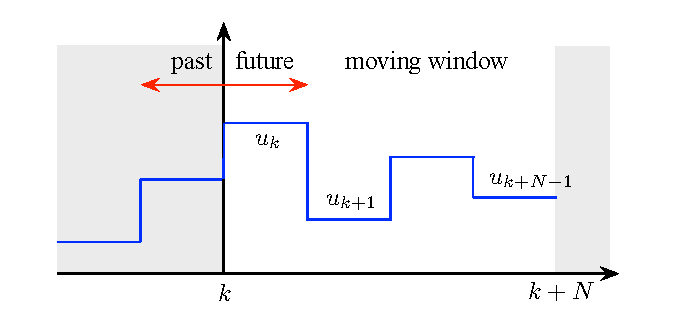
\includegraphics[scale=0.8]{figures/mpc_horizon.eps}
%\caption{Finite-horizon moving window of MPC: at time $k$, the MPC optimization problem is solved for a finite length window of $N$ steps and the first control input $u_k$ is applied; the window then recedes one step forward and the process is repeated at time $k+1$.}
%\captionsetup{justification=centering}
%\label{F:mpc}
%\end{figure}

The objective of the controller is to minimize the energy usage $c^Tu$ while maintaining a desired level of thermal comfort $x_{ref}$.
Therefore, at time step $k$, we solve a continuously linearized MPC problem to determine the optimal sequence of inputs $[u_{\mathrm{k|k}},\dots,u_{\mathrm{k+N-1|k}}]$:
\begin{subequations}
\begin{align}
\text{min } & \sum_{j=1}^{N} ({x}^T_{\mathrm{k+j|k}} - x_{ref}) \mathcal{Q} ({x}_{\mathrm{k+j|k}} - x_{ref}) + c^Tu_{\mathrm{k+j-1}} +  \lambda\epsilon_j\\
\text{s.~t. } & \ \ x_{\mathrm{k+j|k}} =  Ax_{\mathrm{k|k}} + B u_{\mathrm{k+j-1|k}} + B_d d_{\mathrm{k+j-1|k}} \label{SE:mpc1} \\
& \ \ \ \ \ B = B_u + B_{xu}[x_{\mathrm{k|k}}] + B_{du}[d_{\mathrm{k+j-1|k}}] \label{SE:mpc2}\\
& \ \ \ \ \ \ \ \ \ \ \ \ \ \ \ \underline{u} \leq u_{\mathrm{k+j-1|k}} \leq \bar{u}\\ 
& \ \ \ \ \ \ \ \ \ \ \ \ \underline{x}-\epsilon_j \leq x_{\mathrm{k+j|k}} \leq \bar{x} + \epsilon_j\\\
& \ \ \ \ \ \ \ \ \ \ \ \ \ \ \epsilon_j \geq 0, \ j = 1,\dots,N,
\end{align}\label{E:mpc}
\end{subequations} 
\noindent where $\mathcal{Q} \in \R^{12 \times 12}$ has all zeros except at $\mathcal{Q}^{(1,1)}$ corresponding to the zone temperature, $c \in \R^{4}$ is proportional to cost of using each actuator and $\lambda$ penalizes the slack variables.

\subsection{Data Predictive Control}
\label{SS:dpc}
In this section, we explain how DPC can be applied to this case study. We begin with a description of features $\tX$ and output $\tY$ used for training.

\subsubsection{Training Data} 
\label{SSS:dpc_data}

The fundamental reason why DPC  is suitable for such a problem is that when the complexity rises, there is a huge cost to model all the states given by the dynamical system \eqref{E:bilinear1}. For example, states in the bilinear model also include slab temperatures which require modeling of structural and material properties in detail and often we also need to install new sensors to capture additional states. Thus, DPC is based solely on one state of the model i.e. the zone temperature that can be easily measured with a thermostat. This serves as the output variable $\tY$ of interest for which we build $N$ trees and $N$ forests as described in Sec.~\ref{SS:dpcrt} and \ref{SS:dpcrf}, respectively. Therefore, $\tY_{\mathrm{k+j|k}}:=x_{\mathrm{k+j|k}}^1$, where $x^1$ is the first component of $x$.
Next, we define the non-manipulated features $\tX^d_{\mathrm{k|k}}$. At time $k$, for the tree $\mathcal{T}_j$ and the forest $\mathcal{R}_j$, we base these features to include weather disturbances, external disturbances due to occupancy and equipments, and autoregressive terms of the room temperature, i.e.
$\tX^d_{\mathrm{k|k}}:=[ d_{\mathrm{k+j-N|k}} ,\dots,d_{\mathrm{k+j-1|k}}, x_{\mathrm{k|k}}^1,\dots, x_{\mathrm{k-\delta|k}}^1 ]$, where $\delta$ is the order of autoregression.
Finally, the inputs in DPC are exactly same as in MPC. i.e. $\tX^c_{\mathrm{k+j-1|k}}:=u_{\mathrm{k+j-1|k}}$.

The training data in the above format was generated by simulating the bilinear model with rule-based strategies for 10 months in 2007. January and May were deliberately excluded for testing the DPC implementation.

\subsubsection{Optimization} 
\label{SSS:dpc_opt}
For a fair comparison with MPC, we cast DPC optimization problem as follows:
\begin{subequations}
\begin{align}
\text{min } & \sum_{j=1}^{N} {\tY}_{\mathrm{k+j|k}} \mathcal{Q}^{(1,1)} {\tY}_{\mathrm{k+j|k}} + c^T \tX^c_{\mathrm{k+j-1|k}}+  \lambda\epsilon_j\\
\text{s.~t. } & \ \ \ \ \ \tY_{\mathrm{k+j|k}} =  \alpha_j^T \left[1,\tX^c_{\mathrm{k|k}},\dots,\tX^c_{\mathrm{k+j-1|k}} \right]^T \label{SE:dpc}\\
& \ \ \ \ \ \ \ \ \ \ \ \ \ \ \ \underline{\tX}^c \leq \tX^c_{\mathrm{k+j-1|k}} \leq \bar{\tX}^c\\ 
& \ \ \ \ \ \ \ \ \ \ \ \ \underline{\tY}-\epsilon_j \leq \tY_{\mathrm{k+j|k}} \leq \bar{\tY} + \epsilon_j\\\
& \ \ \ \ \ \ \ \ \ \ \ \ \ \ \epsilon_j \geq 0, \ j = 1,\dots,N.
\end{align} \label{E:dpc}
\end{subequations}
\noindent Here $\alpha = \beta$ for DPC-RT and $\alpha = \hat{\Theta}$ for DPC-En.
Note that, \eqref{E:dpc} is DPC analog of \eqref{E:mpc}. The only difference is the state dynamics \eqref{SE:mpc1} and \eqref{SE:mpc2} are now replaced with \eqref{SE:dpc}.

\subsubsection{Validation} 
\label{SSS:dpc_val}

We compare the prediction for the first time step $\tY_{\mathrm{k+1|k}}$ and the 6-hour ahead prediction $\tY_{\mathrm{k+6|k}}$ for a week in the month of May in Fig.~\ref{F:validation}. It is visible how trees have a high variance, and the forests are more accurate. Note that data from January and May was not used for training. The quantitative summary of the accuracy is given in Tab.~\ref{T:validation}. We can see that the random forests are better in all respects.
\begin{table}[h!]
	\centering
	\begin{tabular}{cccc}
		\toprule
		& RMSE & $R^2$ score & EV  \\ 
		\midrule
		tree-$\tY_{\mathrm{k+1|k}}$    &  0.42 &  0.75 & 0.76    \\
		tree-$\tY_{\mathrm{k+6|k}}$  & 0.64 &  0.41  & 0.42 \\
		forest-$\tY_{\mathrm{k+1|k}}$  & 0.29 & 0.87  & 0.88 \\
		forest-$\tY_{\mathrm{k+6|k}}$  & 0.38 & 0.78 & 0.80 \\
		\bottomrule
	\end{tabular}
	\caption{Quantitative comparison of root mean square error (RMSE), $R^2$ score, and explained variance (EV) for trees and forests for different predictions steps.}
	\captionsetup{justification=centering}
	\label{T:validation}
\end{table}

\begin{figure}[h!]
	\centering
	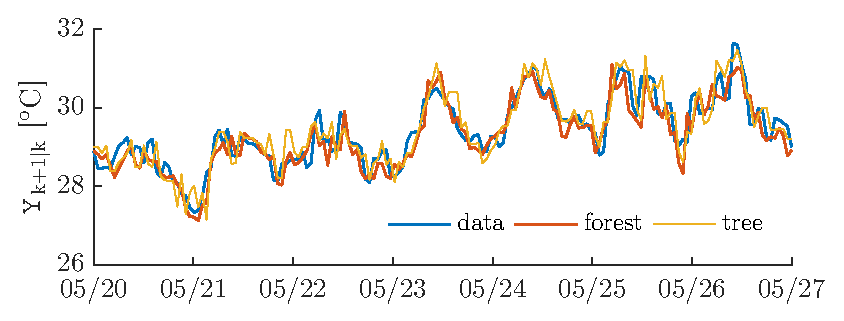
\includegraphics[width=20pc]{figures/validation-s1.eps}
	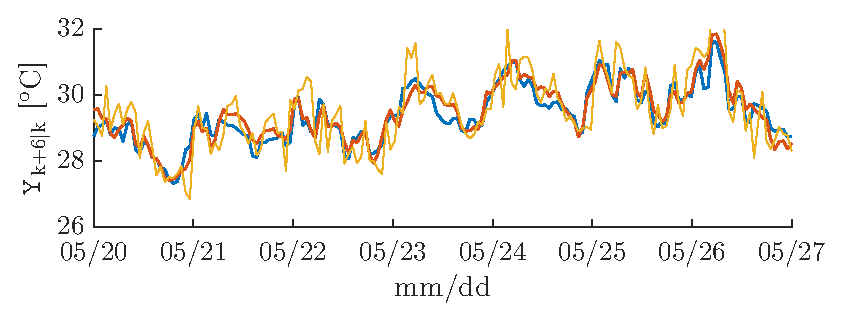
\includegraphics[width=20pc]{figures/validation-s6.eps}
	\caption{Temperature predictions from a tree and a forest for first step prediction (top) and the 6-hour ahead prediction (bottom). Ensemble method shows a relatively higher accuracy.}
	\captionsetup{justification=centering}
	\label{F:validation}
\end{figure}

%\begin{figure}[t!]
%	\centering
%	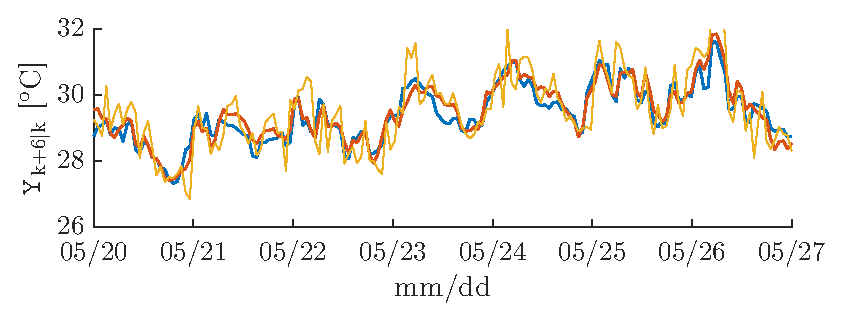
\includegraphics[width=20pc]{figures/validation-s6.eps}
%	\caption{Temperature predictions from a tree and a forest for 6 hour ahead prediction.}
%	\captionsetup{justification=centering}
%	\label{F:validation-s6}
%\end{figure}

\subsection{Comparison}
\label{SS:comp}
We compare the performance of DPC \eqref{E:dpc} against an equivalent MPC formulation \eqref{E:mpc}. The solution obtained from MPC sets the benchmark that we compare to. Note that the MPC implementation uses the exact knowledge of the plant dynamics. Therefore, the associated control strategy is indeed the optimal strategy for the plant.

The performance is compared for 3 days in winter, i.e. January 28-31 and 3 days in summer, i.e. May 1-3. These are shown on the same plots in Figure~\ref{F:comparison}.
The sampling time in the simulations is 1 hr. The control horizon $N$ and the order of autoregression are both 6 hrs. The training procedure required a few minutes in the case of trees and 2 hrs for forests on a Win 10 machine with an i7 processor and 8GB memory.
The cooling usage factor $\mathsf{C}$ is constrained in $[0,1]$, the heat input in $[0,23]\ \mathrm{W/m^2}$, and the room temperature in $[19,25]\ \mathrm{^oC}$ during the winters and $[20,26]\ \mathrm{^oC}$ during the summers.
The optimization is solved using CPLEX \cite{IBM}.

The external disturbances - solar gain, internal gain due to equipment and dry-bulb temperature during the chosen periods are shown in Figure~\ref{F:dist}. The internal gain due to occupancy was proportional to the gain due to equipment. 
The reference temperature is chosen to be 22 $\mathrm{^oC}$. Due to cold weather, which is evident from the dry-bulb temperature, the heating system is switched on during the night to maintain the thermal comfort requirements. When the building is occupied during the day, due to excessive internal gain, the building requires cooling. The lighting in the building is adjusted to meet the minimum light requirements.
The optimal cooling usage factor and the radiator power for MPC, DPC-En and DPC-RT are shown in Figure~\ref{F:control1} and Figure~\ref{F:control2}, respectively. The control strategy with DPC-En shows a remarkable similarity to MPC, switching on/off the equipments at the same time with similar usage. However, the performance with DPC-RT is much different and worse. DPC-RT inherently suffers from high variance which is also evident in the control strategy, thus making it unsuitable for practical purposes. 
Although it seems like that adding the rate constraints to DPC-En would smoothen its behavior, this was avoided because the sampling time of the system is 1 hr which is already too high. The room temperature profile in Figure~\ref{F:state} is close to the reference in the case of DPC-En as well as MPC. 
Figure~\ref{F:obj} shows that the cumulative cost of the objective function is, as expected, minimum for MPC, and a bit higher for DPC-En. The cost for DPC-RT blows up around 12 noon on 30$^{th}$ January as one of the slack variables is non-zero, which happens due to high model inaccuracy.

The quantitative performance comparison is shown in Table~\ref{T:comparison}. MPC tracks the reference more closely at the expense of higher input costs in comparison to DPC-En. The higher cost of the inputs in MPC is also due to lighting. DPC-En explains 70.1\% variation in the optimal control strategies obtained from MPC while DPC-RT explains only 1.8\%. The mean optimal cost of DPC-En is more than MPC, and is maximum for DPC-RT due to a constraint violation.

\begin{table}[h!]
	\centering
	\begin{tabular}{ccccc}
		\toprule
		& explained & mean objective& mean input  & mean  \\
		&  variance$[\mathrm{-}]$ & value $[\mathrm{-}]$ & cost $[-]$ & deviance $[\mathrm{^oC}]$ \\     
		\midrule
		MPC    &  $\mathrm{-}$ &  22.60 & 17.16  &  0.26  \\
		DPC-En   & 70.1\% &  39.26  & 15.12 &  0.48 \\
		DPC-RT  & 1.8\% & 204.55 & 16.84 &  0.57 \\
		\bottomrule
	\end{tabular}
	\vspace{0.2cm}
	\caption{Quantitative comparison of explained variance, mean value of objective function, mean input cost $c^Tu$ and mean deviance from the reference temperature $|\mathsf{T}-\mathsf{T}_{\mathrm{ref}}|$.}
	\captionsetup{justification=centering}
	\label{T:comparison}
\end{table}

\begin{figure}[t!]
	\begin{center}
	\vspace{1.1cm}
	\subfigure[External disturbances: solar gain, internal gain due to equipment and dry-bulb temperature.]{
		\label{F:dist}
		\centering
		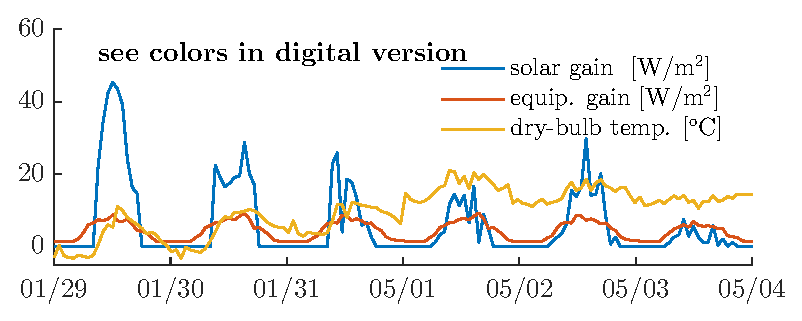
\includegraphics[width=25pc]{figures/disturbances.eps}
	}

	\subfigure[Optimal control input: cooling usage factor $\mathsf{C}$ with  $0 \leq \mathsf{C} \leq 1$. DPC-En generates a control strategy very simular to MPC.]{
		\label{F:control1}
		\centering
		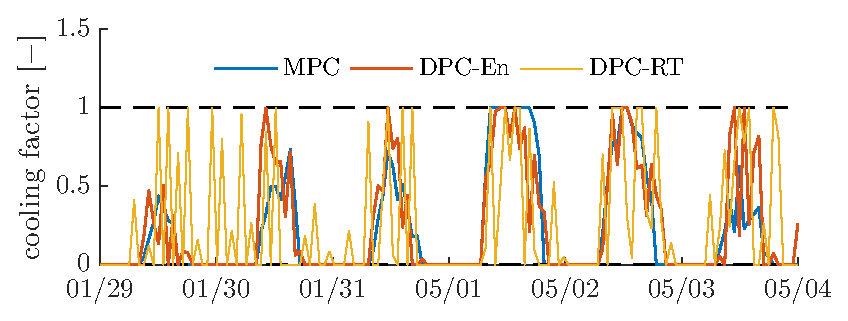
\includegraphics[width=25pc]{figures/input3.eps}
	}

\end{center}
\end{figure}
\begin{figure}[h!]
\begin{center}
	\subfigure[Optimal control input: radiator heat $\mathsf{H}$ with  $0 \leq \mathsf{H} \leq 23 \ \mathrm{W/m^2}$. Again, DPC-En generates a control strategy very simular to MPC.]{
		\label{F:control2}
		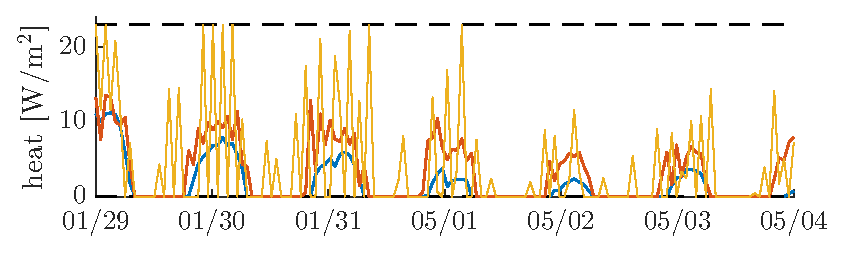
\includegraphics[width=25pc]{figures/input4.eps}
	}

	\subfigure[Room temperature has time varying bounds. When the building is occuped the constraints are relaxed, else $19(20) \leq \mathsf{T}_{\mathrm{in}} \leq 25(26) \ \mathrm{^oC}$ in January(May). MPC and DPC-En are able to track the reference temperature ($22 \ \mathrm{^oC}$) closely.]{
		\label{F:state}
		\centering
		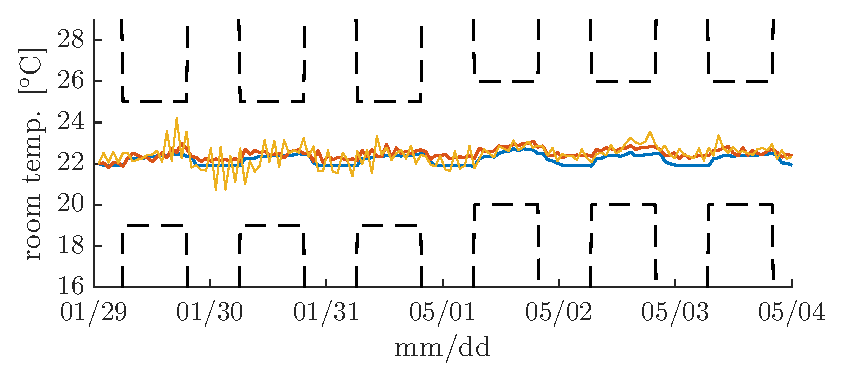
\includegraphics[width=25pc]{figures/state.eps}
	}

	\subfigure[Cumulative optimal cost after solving optimization. MPC serves as the benchmark with the minimum cost, followed by DPC-En and then DPC-RT.]{
		\label{F:obj}
		\centering
		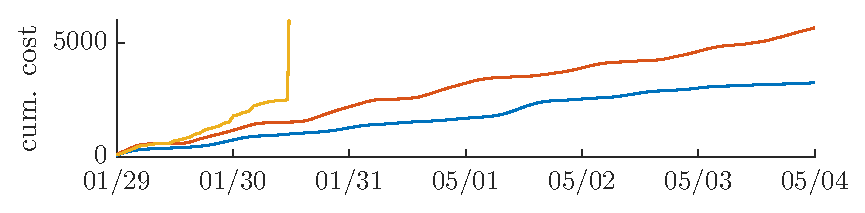
\includegraphics[width=25pc]{figures/cumsumcost.eps}
	}
	\end{center}
	%\vspace{-1cm}
	\caption{Comparison of optimal performance obtained with MPC, DPC-En and DPC-RT for 3 days in January and 3 days in May.}
	\label{F:comparison}
	\captionsetup{justification=centering}
\end{figure}
Thus, we have shown that DPC-En provides a comparable performance to MPC without using the physical model.
However, one major limitation of the bilinear model is that the information about the building power consumption is not available. Much nonlinearities in the system are due to equipment efficiencies which are not considered in the bilinear case but are very important for practical purposes. 

Therefore, our next goal is to apply DPC-En on even more complex and realistic EnergyPlus model for which building a model predictive controller is time and cost prohibitive \cite{Sturzenegger2016}. This is because we would need to model intricate details like the geometry and construction layouts, the equipment design and layout plans, material properties, equipment and operational schedules etc.


